


\begin{figure}[t]
    \centering
    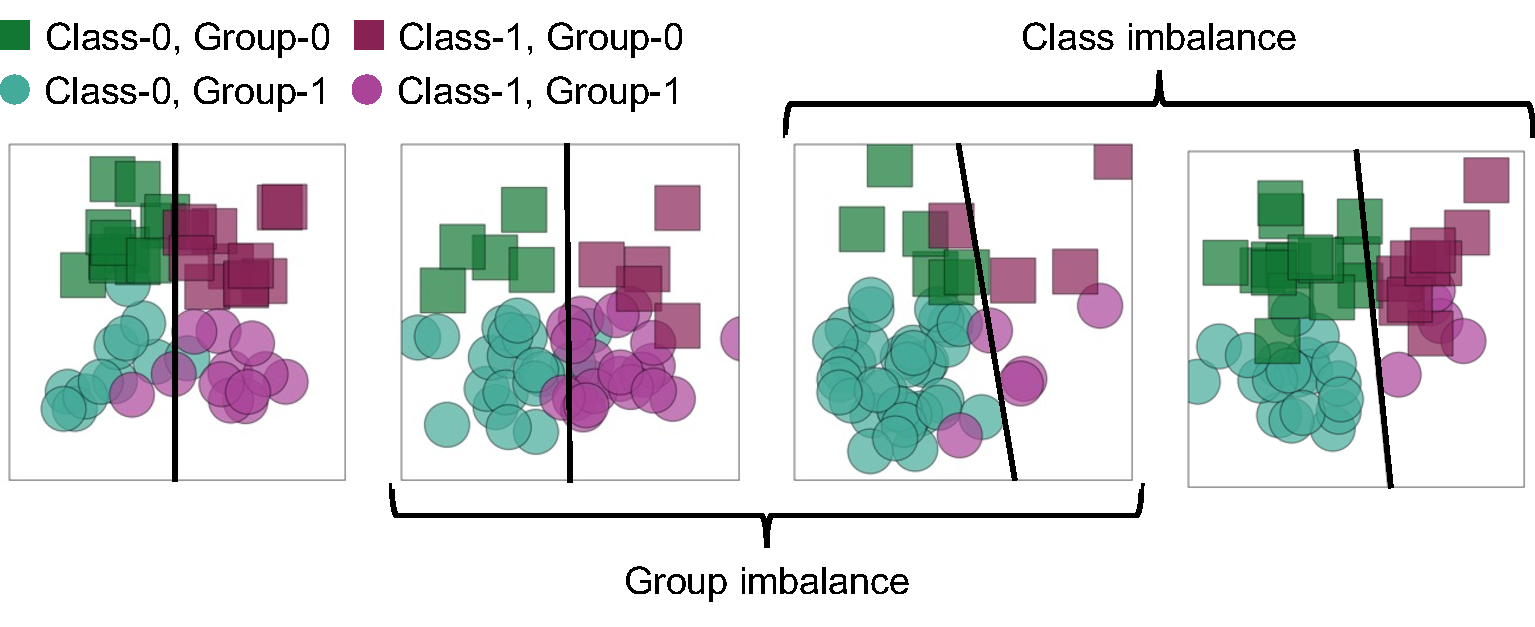
\includegraphics[width=1.0\linewidth]{figures/fairness_toy_exp_2.pdf}
    \caption{\textbf{Influence of the class and group imbalance on classifier during training.} 
    The 2D data are sampled from the normal distributions with four different means and the same covariance. 
    We simulate 4 different experiments with the latent group imbalance (sensitive attributes) by adjusting the number of data in each group.
    The total number of samples is the same.
    We train classifiers for the classes on different imbalance settings and visualize the learned classifiers (bold black lines).
    The fairer the classifiers, the more vertically aligned.
    % When both classes and groups are imbalanced, it yields the most unfair classifier. 
    The classifier trained on the class imbalance is more unfair than the one on the group imbalance.
    % The experiment setting details can be found in the supplementary material.
    }
    \label{fig:fair_toy}
\end{figure}



\begin{table}[]
    \centering
    \begin{subtable}{0.95\linewidth}
        \centering
        \resizebox{\linewidth}{!}{
            \begin{tabular}{lcccc}
            \toprule
            \textbf{Method} & \textbf{Accuracy} & \textbf{DP} & \textbf{ED} & \textbf{EO}\\
            \midrule
            \multicolumn{5}{c}{ResNet18} \\
            \midrule
            % ERM & 93.9 & 0.08174 & 0.0632 & 0.0779\\
            % SYNAuG & 94.0 & 0.06995 & 0.0563 & 0.06825\\
            ERM & 93.9 & 0.0817 & 0.0632 & 0.0779\\
            SYNAuG & \textbf{94.1} & \textbf{0.060} & \textbf{0.0462} & \textbf{0.0434}\\
            \midrule
            \multicolumn{5}{c}{ResNet50} \\
            \midrule
            % ERM & 94.0 & 0.07272 & 0.0585 & 0.07269\\
            % SYNAuG & \textbf{94.1} & \textbf{0.06138} & \textbf{0.04723} & \textbf{0.05885}\\
            ERM & 94.0 & 0.07272 & 0.0585 & 0.07269\\
            SYNAuG & \textbf{94.4} & \textbf{0.05432} & \textbf{0.03936} & \textbf{0.05472}\\
            \bottomrule
           \end{tabular}
        }
    \caption{\textbf{Fairness performance.}}
    \vspace{2mm}
    \label{tab:fairness_1}
    \end{subtable}

    \begin{subtable}{0.95\linewidth}
        \centering
        \resizebox{\linewidth}{!}{
            \begin{tabular}{lcccc}
            \toprule
            \textbf{Method} & \textbf{Accuracy} & \textbf{DP} & \textbf{ED} & \textbf{EO}\\
            \midrule
            ERM & 93.9 & 0.08174 & 0.0632 & 0.0779\\
            + Group-DRO & 93.9 & 0.07266 & 0.05819 & 0.06954\\
            + RS & 93.8 & \textbf{0.0636} & \textbf{0.04663} & \textbf{0.05808} \\
            \midrule
            SYNAuG & \textbf{94.0} & 0.06995 & 0.0563 & 0.06825\\
            + Group-DRO & 93.9 & 0.0711 & 0.05433 & 0.07045\\
            + RS & 93.6 & 0.06786  & 0.06439 & 0.0812 \\
            \bottomrule
           \end{tabular}
        }
       \caption{\textbf{Ablation with other algorithms}}
       \vspace{2mm}
       \label{tab:fairness_2}
   \end{subtable}

    \begin{subtable}{0.95\linewidth}
        \centering
        \resizebox{\linewidth}{!}{
            \begin{tabular}{lcccc}
            \toprule
            \textbf{Method} & \textbf{Accuracy} & \textbf{DP} & \textbf{ED} & \textbf{EO}\\
            \midrule
            ERM & 93.9 & 0.08174 & 0.0632 & 0.0779\\
            + Mixup & 93.9 & 0.07266 & 0.05819 & 0.06954\\
            + CutMix & 94.7 & 0.08265 & 0.06245 & 0.08333\\
            \midrule
            SYNAuG& 94.0 & 0.06995 & 0.0563 & 0.06825\\
            + Mixup & 94.2 & \textbf{0.064} & \textbf{0.03793} & \textbf{0.04658}\\
            + CutMix & \textbf{94.9} & 0.0743 & 0.04745 & 0.06319\\
            \bottomrule
           \end{tabular}
        }
       \caption{\textbf{Augmentation abalation}}
       \vspace{2mm}
       \label{tab:fairness_3}
   \end{subtable}

    \begin{subtable}{0.95\linewidth}
        \centering
        \resizebox{\linewidth}{!}{
            \begin{tabular}{lcccc}
            \toprule
            \textbf{Method} & \textbf{Accuracy} & \textbf{DP} & \textbf{ED} & \textbf{EO}\\
            \midrule
            SYNAuG$^*$ & \textbf{94.0} & 0.07342 & 0.05805 & 0.07253\\ 
            SYNAuG & \textbf{94.0} & \textbf{0.06995} & \textbf{0.0563} & \textbf{0.06825}\\ 
            \bottomrule
            \addlinespace[0.2mm]
            \multicolumn{5}{l}{*Not use the sensitivity attribute}
           \end{tabular}
        }
       \caption{\textbf{Sensitivity abalation}}
       \label{tab:fairness_4}
   \end{subtable}
   
   \caption{\textbf{Fairness performance.} 
   (a) accuracy and model fairness results of our SYNAuG, 
   (b) compatibility with other fairness algorithms, Group-DRO and Re-Sampling (RS), 
   (c) ablation study with data augmentation, Mixup and Cuxmix, 
   and (d) ablation study using the prior about sensitive attribute. \textbf{Bold} means the highest accuracy and the best fairness performance in a table. 
   Higher is better in accuracy, and lower is better in fairness metrics.}
   \label{tab:temps}
\end{table}

Group imbalance stands for the data imbalance between groups, such as ethnicity. 
We empirically observe that the group imbalance with the class imbalance amplifies 
% yields
unfair classifiers, as shown in \Fref{fig:fair_toy}.
The class imbalance affects the unfair classifier more than the group imbalance.
Both class and group imbalance contribute to the unfair classifier.

Model fairness, one of the problems caused by group imbalance, is essential to prevent unexpected social confusion.
Fairness metrics have been proposed to measure the fairness performance of models:
Demographic Parity (DP) $=\max_z|P(y_p{=}1|z) {-} P(y_p{=}1)|$ \cite{10.1145/2783258.2783311},
Equal Opportunity (EO) $=\max_{z_i, z_j, y, y_p}|P_{z_i}(y_p|y) {-} P_{z_j}(y_p|y)|$ \cite{hardt2016equality, jung2022learning},
and Equalized Odds (ED) $=\max_{z, y, y_p}|P(y_p|z, y) {-} P(y_p|y)|$ \cite{hardt2016equality}, where $y_p$ is the prediction, $y$ is the class label, and $z$ is the sensitive attribute.
These metrics are based on the difference in the performance of the learned classifiers depending on groups, \ie, the sensitive attributes.
Lower values of fairness metrics indicate that the model is fairer.


% \begin{table*}[t]
%     \begin{subtable}[b]{0.49\linewidth}
%         \centering
%         \resizebox{\linewidth}{!}{
%             \begin{tabular}{lcccc}
%             \toprule
%             Method & Accuracy & DP & ED & EO \\
%             \midrule
%             % ERM & 93.9 & 0.08174 & 0.0632 & 0.0779\\
%             % SYNAuG$^*$ & \textbf{94.0} & 0.07342 & 0.05805 & 0.07253\\ ICCV 
%             % SYNAuG & \textbf{94.0} & \textbf{0.06995} & \textbf{0.0563} & \textbf{0.06825}\\ ICCB
%             ERM & 93.9 & 0.0817 & 0.0632 & 0.0779\\
%             SYNAuG & \textbf{94.1} & \textbf{0.060} & \textbf{0.0462} & \textbf{0.0434}\\
%             \bottomrule
%            \end{tabular}}
%        \caption{\textbf{Balancing with SYNAuG.}}
%        \label{tab:fair_syn}
%     \end{subtable}
%     \hfill
%     \begin{subtable}[b]{0.49\linewidth}
%         \centering
%         \resizebox{\linewidth}{!}{
%             \begin{tabular}{lcccc}
%             \toprule
%             Method & Accuracy & DP & ED & EO\\
%             \midrule
%             ERM & 93.9 & 0.08174 & 0.0632 & 0.0779\\
%             + Groupp-DRO & 93.9 & 0.07266 & 0.05819 & 0.06954\\
%             + RW & 93.8 & 0.0636 & 0.04663 & 0.05808 \\
%             \midrule
%             SYNAuG & \textbf{94.0} & \textbf{0.06995} & 0.0563 & \textbf{0.06825}\\
%             + Group-DRO & 93.9 & 0.0711 & \textbf{0.05433} & 0.07045\\
%             + RW & 93.6 & 0.06786  & 0.06439 & 0.0812 \\
%             \bottomrule
%            \end{tabular}
%         }
%        \caption{\textbf{Algorithm generalization}}
%        \label{tab:week2}
%    \end{subtable}
   
%     \begin{subtable}[b]{0.49\linewidth}
%         \centering
%         \resizebox{\linewidth}{!}{
%             \begin{tabular}{lcccc}
%             \toprule
%             Method & Accuracy & DP & ED & EO\\
%             \midrule
%             ERM & 93.9 & 0.08174 & 0.0632 & 0.0779\\
%             + Mixup & 93.9 & 0.07266 & 0.05819 & 0.06954\\
%             + CutMix & 94.7 & 0.08265 & 0.06245 & 0.08333\\
%             \midrule
%             SYNAuG& 94.0 & 0.06995 & 0.0563 & 0.06825\\
%             + Mixup & 94.2 & \textbf{0.064} & \textbf{0.03793} & \textbf{0.04658}\\
%             + CutMix & \textbf{94.9} & 0.0743 & 0.04745 & 0.06319\\
%             \bottomrule
%            \end{tabular}
%         }
%        \caption{\textbf{Augmentation generalization}}
%        \label{tab:week2}
%    \end{subtable}
%    \hfill
%    \begin{subtable}[b]{0.49\linewidth}
%         \centering
%         \resizebox{\linewidth}{!}{
%             \begin{tabular}{lcccc}
%             \toprule
%             Method & Accuracy & DP & ED & EO\\
%             \midrule
%             \multicolumn{5}{c}{ResNet18} \\
%             \midrule
%             % ERM & 93.9 & 0.08174 & 0.0632 & 0.0779\\
%             % SYNAuG & 94.0 & 0.06995 & 0.0563 & 0.06825\\
%             ERM & 93.9 & 0.0817 & 0.0632 & 0.0779\\
%             SYNAuG & \textbf{94.1} & \textbf{0.060} & \textbf{0.0462} & \textbf{0.0434}\\
%             \midrule
%             \multicolumn{5}{c}{ResNet50} \\
%             \midrule
%             % ERM & 94.0 & 0.07272 & 0.0585 & 0.07269\\
%             % SYNAuG & \textbf{94.1} & \textbf{0.06138} & \textbf{0.04723} & \textbf{0.05885}\\
%             ERM & 94.0 & 0.07272 & 0.0585 & 0.07269\\
%             SYNAuG & \textbf{94.4} & \textbf{0.05432} & \textbf{0.03936} & \textbf{0.05472}\\
%             \bottomrule
%            \end{tabular}
%         }
%        \caption{\textbf{Architecture generalization.}}
%        \label{tab:week2}
%    \end{subtable}
     
%      \caption{\textbf{Fairness performance.} (a) shows the result of our SYNAuG, (b) the experiments with Group-DRO, (c) the experiments with data augmentation, Mixup and Cuxmix, and (d) experiments with deeper architecture, ResNet50. \textbf{Bold} means the highest accuracy and the best fairness performance in a table. Higher is better in accuracy, and lower is better in fairness metrics.}
%      \label{tab:temps}
%      \vspace{-5mm}
% \end{table*}

\paragraph{Experiments on UTKFace.}
We employ UTKFace~\cite{zhifei2017cvpr} composed of 23,708 images with age, gender, and race labels.
We use race annotation as a sensitive attribute (group label) and gender as the class label.
For SYNAuG, we augment the data to mitigate the class imbalance across the sensitive attribute;
the female and male ratio of each sensitive attribute becomes equal.
%We evaluate the accuracy and fairness metric from the model at the last epoch.
% 바로 뒤에는 fairness metrics 로 쓰셔서 혹시 몰라 적어놓겠습니다.
We evaluate the accuracy and fairness metrics from the model at the last epoch.
Firstly, we validate the effectiveness of SYNAuG in \Tref{tab:fairness_1}.
The result shows that SYNAuG outperforms ERM in accuracy and fairness metrics on both ResNet18 and ResNet50.

\paragraph{Ablation with other algorithms.} 
%In \Tref{tab:fairness_2}, we experiment with the algorithm explaining the sensitive attributes, Group-DRO~\cite{sagawa2019distributionally} and Re-Sampling (RS).
% 바로 위와 같은 이유로 달아 놓겠습니다.
In \Tref{tab:fairness_2}, we evaluate the performance of the two algorithms Group-DRO~\cite{sagawa2019distributionally} and Re-Sampling (RS).
Note that we do not apply Mixup and fine-tuning in this experiment.
Group-DRO and RS improve the fairness metrics of ERM at the same time.
SYNAuG without Group-DRO outperforms the accuracy and two fairness metrics, ED and EO, compared to Group-DRO.
Developing a fairness algorithm with synthetic data might be a promising direction toward a fair model.

\paragraph{Augmentation ablation.} 
In \Tref{tab:fairness_3}, we compare the effect of data augmentations, Mixup~\cite{zhang2017mixup} and CutMix~\cite{yun2019cutmix}.
In this ablation study, we do not apply fine-tuning for clear comparison.
Both augmentations improve the accuracy of ERM; Mixup also works 
% does
in the fairness metrics.
Compared to ERM with Mixup, SYNAuG shows higher accuracy and better fairness metrics.
% EO metric, but underperforms in the other two metrics.
SYNAuG with Mixup outperforms more in accuracy and fairness metrics compared to ERM with Mixup.


\paragraph{No prior of sensitive attribute.}
Labeling sensitive attributes might be expensive.
In this ablation study, we augment the synthetic data to mitigate the class imbalance regardless of sensitive attributes.
We denote this setting as SYNAuG$^*$.
As shown in \Tref{tab:fairness_4}, SYNAuG$^*$ shows better fairness metrics compared to ERM.
However, exploiting the knowledge of sensitive attributes is more effective.

\paragraph{Summary.} 
Class imbalance in fairness can easily cause an unfair model.
This motivates us to balance the class imbalance using synthetic data before tackling fairness directly.
We observe that the synthetic data improves both model accuracy and fairness simultaneously.
The experimental results also demonstrate that SYNAuG is compatible with other training algorithms, data augmentation, and network architecture.


